\section{Задание 4. Поверхности второго порядка}

\textbf{Условие.}

Даны $T_1$ и $T_2$ – тела, ограниченные поверхностями не выше второго порядка.
Тело $T_1$ изображено своим сечением в плоскости $Oyz$. Проекцией тела на плоскость $Oxz$ является круг.
Тело $T_2$ задано уравнениями ограничивающих поверхностей.

\begin{enumerate}
    \item Запишите уравнения и названия поверхностей, ограничивающих тело $T_1$.
    \item Изобразите тело $T_2$ и его проекции на координатные плоскости.
\end{enumerate}
\vspace{3mm}

\begin{multicols}{2}
    \begin{enumerate}
        \begin{center}
            \item Тело $T_1$: \vspace{2mm}

            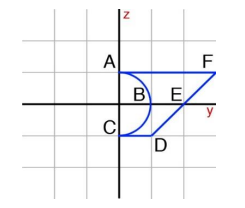
\includegraphics{images/4a1}

            \item Тело $T_2$: \vspace{2mm}

            \begin{cases}
                y + \sqrt{1 - x^2 - z^2} = 0,\\
                y + 2\sqrt{x^2 + z^2} = 2
            \end{cases}\\
        \end{center}
    \end{enumerate}
\end{multicols}

\vspace{10mm}
\textbf{Решение.}

\begin{enumerate}
    \item Тело $T_1$:
    \vspace{2mm}

    \begin{center}
        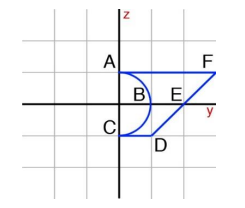
\includegraphics[width=5cm]{images/4a1}
    \end{center}

    \vspace{2mm}

    Так как проекция тела на плоскость $Oxz$ является кругом, то это может соответствовать боковой поверхности цилиндра $x^2 + z^2 = 1$ - радиус равен 1, т. к. $|AC| = 2$

    Отрезку $DF$ на проекции может соответствовать плоскость $y - z = 2$.

    Полуокружности $ABC$ соответствует боковая поверхность цилиндра $y^2 + z^2 = 1$ - радиус равен 1, т. к. $|AC| = 2$

    Так будут выглядеть эти поверхности в Desmos: \\(источник: \url{https://www.desmos.com/3d/6d4203791f})

    \begin{center}
        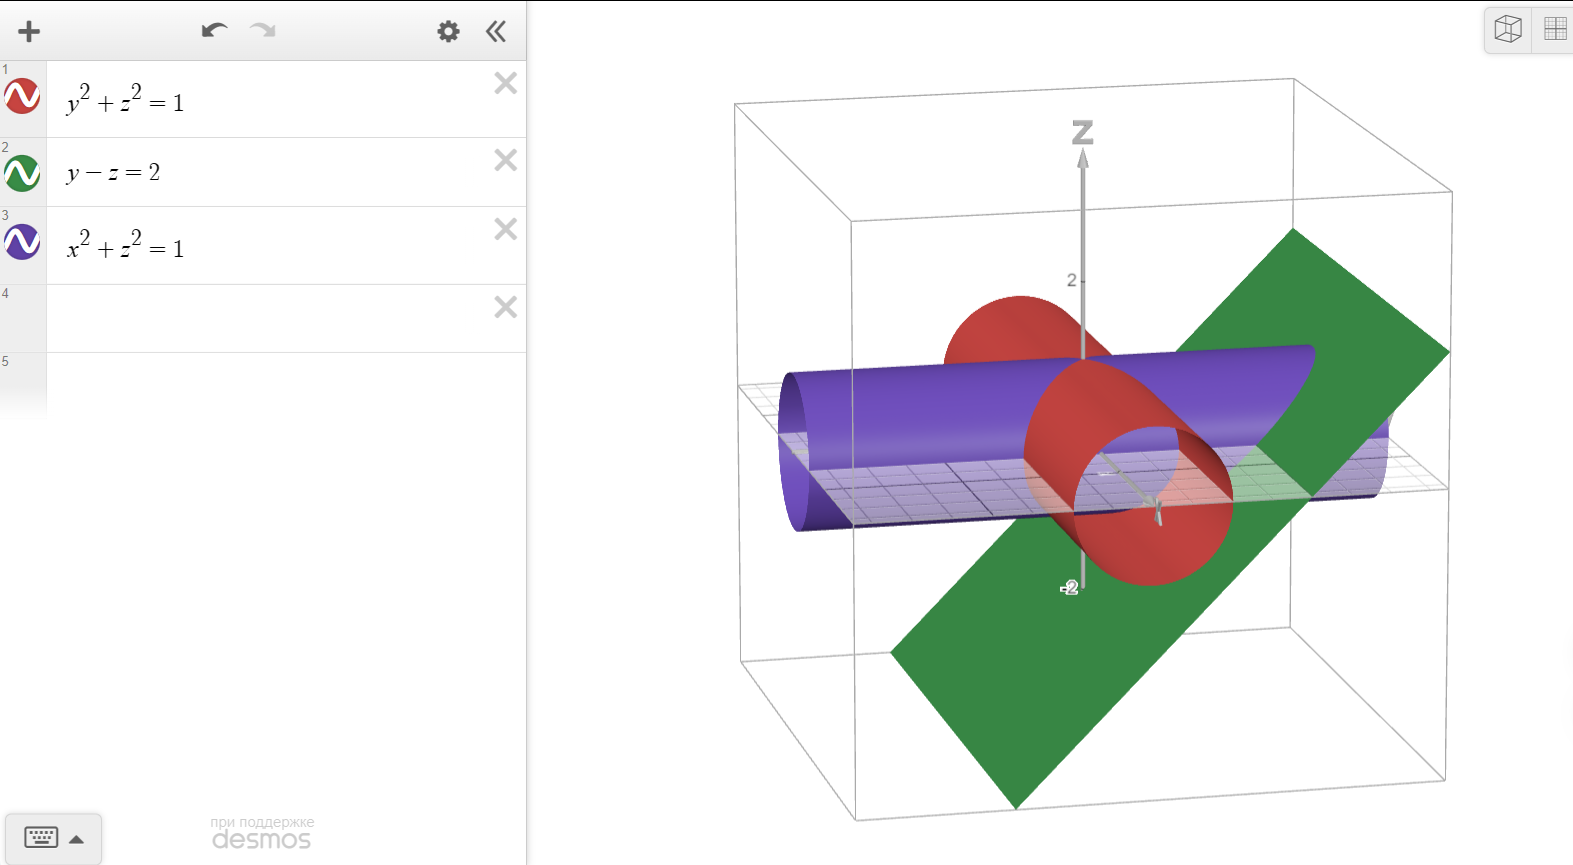
\includegraphics[width=15cm]{images/4a2}
    \end{center}

    \item Тело $T_2$:
    \vspace{2mm}

    \begin{cases}
        y + \sqrt{1 - x^2 - z^2} = 0,\\
        y + 2\sqrt{x^2 + z^2} = 2
    \end{cases}\\

    \vspace{2mm}

    Так будут выглядеть эти поверхности в Desmos: \\ (источник: \url{https://www.desmos.com/3d/f37ac1a585})

    \begin{center}
        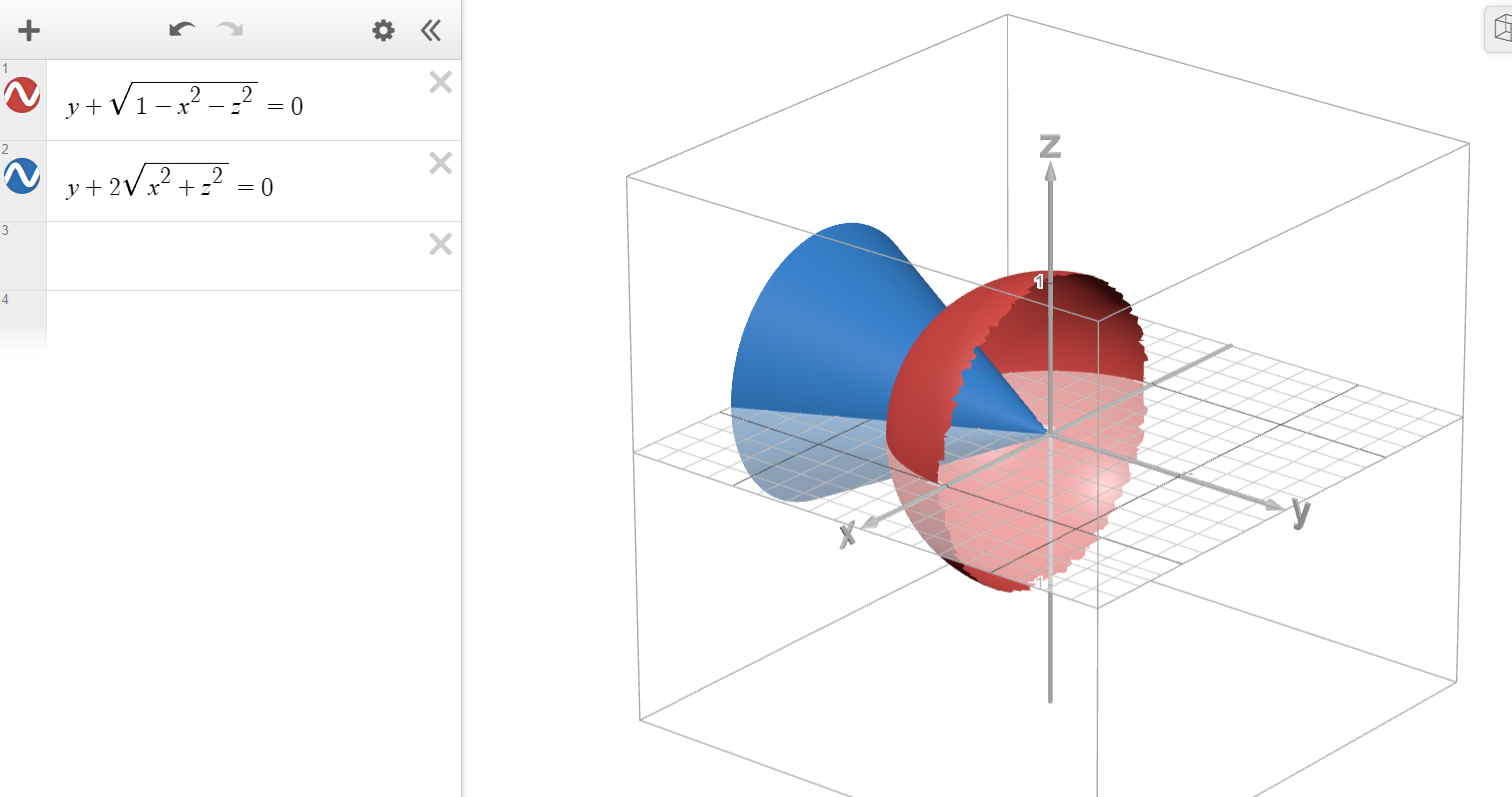
\includegraphics[width=15cm]{images/4b1}
    \end{center}

    Как можно заметить, тело, ограниченное этими поверхностями, является сектором сферы радиусом 1

    Вот его проекции на плоскости $Oxy$ и $Oxz$ (зеленым обведены контуры тела):

    \begin{center}
        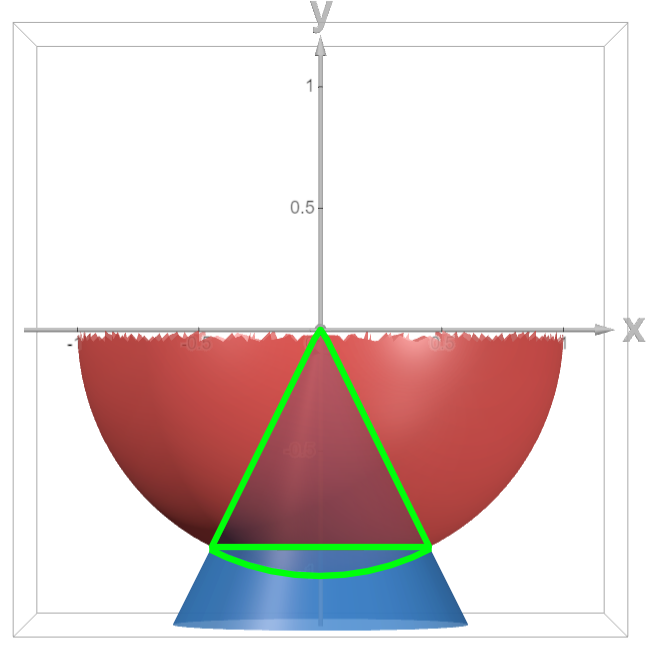
\includegraphics[width=7.5cm]{images/4b2}
        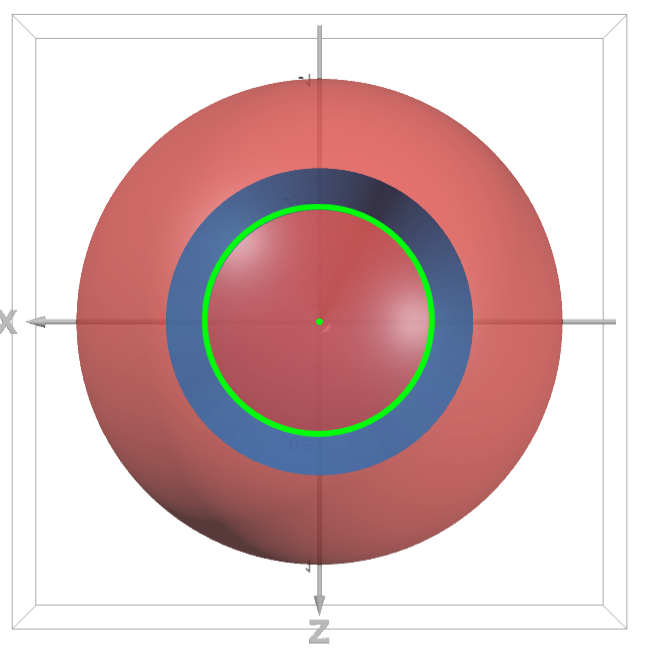
\includegraphics[width=7.5cm]{images/4b3}
    \end{center}

\end{enumerate}

\clearpage
